\section{28 de enero de 2021}

\begin{definition}
Sea $x\in M$ (espacio métrico), entonces cualquier conjunto que contiene un abierto $A\ni x\in A$ es una vecindad de $x$.

\begin{center}
    

\tikzset{every picture/.style={line width=0.75pt}} %set default line width to 0.75pt        

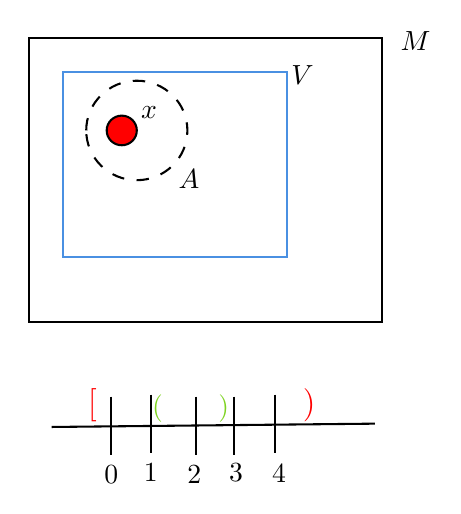
\begin{tikzpicture}[x=0.75pt,y=0.75pt,yscale=-1,xscale=1]
%uncomment if require: \path (0,300); %set diagram left start at 0, and has height of 300

%Shape: Rectangle [id:dp5325951477231496] 
\draw   (31,43.81) -- (201.19,43.81) -- (201.19,180.4) -- (31,180.4) -- cycle ;
%Shape: Rectangle [id:dp6308620272255319] 
\draw  [color={rgb, 255:red, 74; green, 144; blue, 226 }  ,draw opacity=1 ] (47.3,59.84) -- (155.54,59.84) -- (155.54,149.14) -- (47.3,149.14) -- cycle ;
%Shape: Ellipse [id:dp09032950096806747] 
\draw  [dash pattern={on 4.5pt off 4.5pt}] (58.71,88.14) .. controls (58.71,74.9) and (69.62,64.17) .. (83.08,64.17) .. controls (96.54,64.17) and (107.45,74.9) .. (107.45,88.14) .. controls (107.45,101.37) and (96.54,112.1) .. (83.08,112.1) .. controls (69.62,112.1) and (58.71,101.37) .. (58.71,88.14) -- cycle ;
%Shape: Ellipse [id:dp677270653778341] 
\draw  [fill={rgb, 255:red, 255; green, 0; blue, 0 }  ,fill opacity=1 ] (68.57,88.14) .. controls (68.57,84.2) and (71.82,81) .. (75.83,81) .. controls (79.83,81) and (83.08,84.2) .. (83.08,88.14) .. controls (83.08,92.08) and (79.83,95.27) .. (75.83,95.27) .. controls (71.82,95.27) and (68.57,92.08) .. (68.57,88.14) -- cycle ;
%Straight Lines [id:da8462026494214948] 
\draw    (42,231) -- (197.8,229.4) ;
%Straight Lines [id:da36445047109408835] 
\draw    (70.8,216.4) -- (70.8,244.4) ;
%Straight Lines [id:da354987556770879] 
\draw    (89.8,215.4) -- (89.8,243.4) ;
%Straight Lines [id:da777575302939591] 
\draw    (111.8,216.4) -- (111.8,244.4) ;
%Straight Lines [id:da7237425422785222] 
\draw    (129.8,216.4) -- (129.8,244.4) ;
%Straight Lines [id:da6947724696435326] 
\draw    (149.8,215.4) -- (149.8,243.4) ;

% Text Node
\draw (208.65,39.12) node [anchor=north west][inner sep=0.75pt]    {$M$};
% Text Node
\draw (83.68,75.19) node [anchor=north west][inner sep=0.75pt]    {$x$};
% Text Node
\draw (101.76,105.41) node [anchor=north west][inner sep=0.75pt]    {$A$};
% Text Node
\draw (156.04,55.15) node [anchor=north west][inner sep=0.75pt]    {$V$};
% Text Node
\draw (66,248.1) node [anchor=north west][inner sep=0.75pt]    {$0$};
% Text Node
\draw (85,247.1) node [anchor=north west][inner sep=0.75pt]    {$1$};
% Text Node
\draw (106,248.1) node [anchor=north west][inner sep=0.75pt]    {$2$};
% Text Node
\draw (126,247.1) node [anchor=north west][inner sep=0.75pt]    {$3$};
% Text Node
\draw (146.8,247.5) node [anchor=north west][inner sep=0.75pt]    {$4$};
% Text Node
\draw (58,210.9) node [anchor=north west][inner sep=0.75pt]  [font=\large,color={rgb, 255:red, 255; green, 0; blue, 0 }  ,opacity=1 ] [align=left] {[ \ \ \ \ \ \ \ \ \ \ \ \ \ \ \ \ \ \ )};
% Text Node
\draw (89,213.9) node [anchor=north west][inner sep=0.75pt]  [color={rgb, 255:red, 126; green, 211; blue, 33 }  ,opacity=1 ] [align=left] {( \ \ \ \ \ )};


\end{tikzpicture}
\end{center}
\end{definition}

\begin{definition}
Un punto $x\in M$ es un punto interior de un conjunto $A\subseteq M$, si $A$ es una vecindad de $x$. 
\end{definition}

\begin{example}
\begin{itemize}
    \item $[0,1], x=0$ y $x=1$ no son puntos interiores. El resto de puntos de $[0,1)$ son puntos interiores de $[0,1]$
    \item $I=(0,1)$, todos son puntos interiores. 
    \item $\mathbb{R}\cap \mathbb{Z}\subseteq\mathbb{R}$
    %grafica
    $$\implies \mathbb{R}\cap \mathbb{Z}$$
    no tiene puntos interiores. 
    \marginnote{A cualquier conjunto no vacío se le puede dotar de una métrica. 
    $A,d\implies d(x,y)\begin{cases}1,x\neq 1\\ 0,x=0\end{cases}$}
\end{itemize}
\end{example}

\marginnote{Punto interior, por lo menos una bola abierta contenida en $A$}
\begin{definition}
Un punto $x\in M$ es un punto de acumulación (cluster) o punto límite de un conjunto $A\subseteq M$, si cada vecindad de $x$ contiene al menos un punto de $A$ diferente de $x$. Es decir, si 
$$B_r(x)-\{x\})\cap A\neq \emptyset,\forall r>0$$
\begin{example}
$A=\{1,1/2,1/3,...,1/n,...\}\subseteq \mathbb{R}\implies x=0$ es un punto de acumulación de $A$. 
%Grafico 
\end{example}
\end{definition}

\begin{definition}
\begin{enumerate}
    \item El conjunto de todos los puntos interiores de $A$ se llama interior de $A$. (Notación: $A^{0}$ o $int(A)$. %Grafico 
    Es decir, $$int(A)=\bigcup_{U\subset A, \text{u es abierto}}\mathcal{U}$$
    i.e. $int(A)$ es el abierto más grande contenido. \begin{example}
\begin{enumerate}
    \item $int[0,1]=(0,1)$
    \item $int \mathbb{R}\cap \mathbb{Z}=\emptyset$
    \item $int\mathbb{R}^n=\mathbb{R}^n$
    \item $A$ es un conjunto abierto ssi $A=int(A)$
\end{enumerate}
\end{example}
\item La cerradura de $A$ es el conjunto: $$\Bar{A}:=\bigcap_{A\subset F, \text{F cerrado}}$$\begin{remark}
\begin{enumerate}
    \item $\Bar{A}$ es cerrado
    \item $\Bar{A}$ es el cerrado más pequeño que contiene a $A$.
    \item $A$ es cerrado ssi $A=\Bar{A}$
    \item Si $F$ es un cerrado que contiene a $A\implies A\subset \Bar{A}\subset F$
\end{enumerate}
\end{remark}
\item La frontera de $A$ (denotada $bd(A)$ o $\partial A$) Se define: 
$$\partial A:= \Bar{A}-int(A)$$
\begin{example}
Sea$I=[0,1]\implies \Bar{I}=[0,1]\implies (0,1)\implies \partial A=\Bar{I}-int(A)=\{0,1\}$
\end{example}
\item El conjunto de todos los puntos de acumulación de un conjunto $A$ se llama conjunto derivado de $A$. Notación: $A'$
\end{enumerate}
\end{definition}


\begin{proposition}
\begin{enumerate}
    \item Si $A\subset B\implies A'\subset B'$
    \begin{proof}
    Sea $x\in A'$ (i.e. $x$ es un punto de acumulación de $A$). $\implies \forall $ abierto $G\ni x\in G$, se tiene que $$(G-\{x\})\cap A\neq \emptyset $$
    \marginnote{$$A\subset B$$ 
    $$C\subset D$$
    $$\implies A\cap C\subset B\cap D$$}
    Como $A\subset B\implies (G-\{x\}\cap A\subset (G-\{x\})\cap B$
    
    $$\implies \emptyset\neq (G-\{x\})\cap A\subset (G-\{x\})\cap B$$
    $$(G-\{x\})\cap B\neq \empty,\forall G\ni x\in G\implies x\in B'$$
    \end{proof}
    
    \item $(A\cup B)'=A'\cup B'$
    \begin{proof}
    \begin{itemize}
        \item (De ida) Sabemos que $A\subset A\cup B$ y $B\subset A\cup B$ $\implies A'\subset (A\cup B)'$ y $B'\subset (A\cup B)'$
        $$\implies A'\cup B'\subset (A\cup B)'$$
        \item (De regreso) $(A\cup B)'\subset A'\cup B'$\newline 
        $\longleftrightarrow$ Si $x\in (A\cup B)'\implies x\in A'\cup B'$\newline 
        $\Longleftrightarrow$ Si $x\not\in A'\cup B'\implies x\not\in (A\cup B)'$\newline 
        $\implies$ Como $x\not\in A'\implies\exists G$, abierto, tal que $G\cap A\subset \{x\}$\footnote{$G\cap A=\emptyset$ o $G\cap A=\{x\}$ (no)}\newline 
        Como $x\not\in B'\implies \exists H$, abierto, tal que $H\cap A\subset \{x\}$. Nótese que $G\cap H$ es abierto. Entonces, $x\in G\cap H$, y $(G\cap H)\cap (A\cup B)=(G\cap H\cap A)\cup (G\cap H\cap B)\subset \{x\}\cup \{x\}=\{x\}$\newline 
        $\implies x\not\in (A\cup B)'\implies$ si $x\not\in A'\cup B'\implies x\in (A\cup B)'\implies (A\cup B)\subset A'\cup B'\implies (A\cup B)'=A'\cup B'$
        
        
    \end{itemize}
    \end{proof}
\end{enumerate}
\end{proposition}


